\chapter{Adaptive Control Derivation}\label{ch:derivation}

The chapter will outline the various derivations for controllers used in this research.  The controllers designed in this research was simplified assuming generic dynamics of the plant.  For example, the coupling inherent in lateral fixed wing aerodynamics is assumed to be negligible.  With this assumption, each controller is assumed to be \ac{SISO} to reduce complexity.

\section{Preliminaries}\label{preliminaries}
This thesis uses the following notation, nomenclature, and fundamental equations of motion for fixed wing rigid body aerodynamics.

\subsection{Kinematics}
The following is the nomenclature that will be used to describe the kinematic equations.  Euler angles for pitch $(\theta)$, roll $(\phi)$, and yaw $(\psi)$ will have the units of radians.  The following Figure~\ref{fig:reference_frame} illustrates the \ac{NED} reference frame definitions used for body rotational rates about the $x$ axis $(p)$, $y$ axis $(q)$, and the $z$ axis $(r)$ as well as the body velocities in the $x$ axis $(u)$, $y$ axis $(v)$, and the $z$ axis $(w)$.

\subsection{First Order Model}
The following nomenclature will be used to illustrate the modeling of first order systems where $\dot{x}$ is the time derivative of the state, A is the Hurwitz matrix, B is the input matrix, and u is the input vector.
\begin{equation}
\dot{x}(t)=Ax(t)+Bu(t)
\end{equation}
Often times in this thesis, B will be set equal to A.  This is to ensure the DC gain is unity when desired.

\begin{figure}[!h]
 \centering
  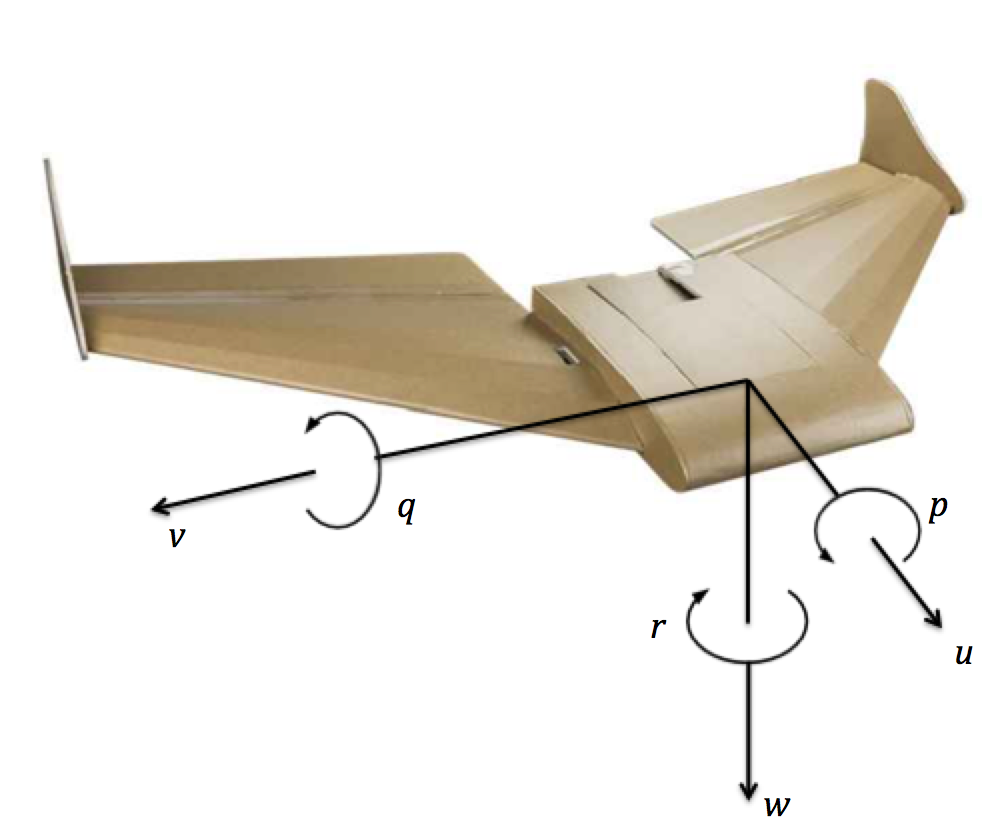
\includegraphics[width=0.65\textwidth]{body_frame_rotations.png}
  \caption{Reference frame - body rates and velocities}
  \label{fig:reference_frame}
\end{figure}

\section{$\mathcal{L}$1 Adaptive Control}
The controller architecture was assumed to be \ac{SISO} for the pitch and roll channels.  This is a fairly gross assumption, but drastically simplifies the controller and for most aircraft will produce adequate rejection to aerodynamic coupling.  The desired channels to be controlled were pitch rate $(q)$ and roll rate $(p)$.  These values were measured by the \ac{IMU} and reported in radians per second.

In this implementation of the $\mathcal{L}$1 adaptive controller, the desired state $x$ to be controlled will be and individual body rate (\eg $q$, $p$).
The following is an example of the controller implemented using a simplified pitch rate model.
\begin{equation}
\dot{q}=Aq+Bq_{cmd}
\end{equation}
where: 
\begin{itemize}
	\item[] $\dot{q}$ = time derivative of pitch rate, radians per $\sq{second}$
	\item[] $A$ = Hurwitz matrix
	\item[] $q$ = pitch rate, radians per second
	\item[] $B$ = input matrix
	\item[] $q_{cmd}$ = pitch rate command, radians per second
\end{itemize}
The values for A and B are usually assumed to be time invariant.  One can assume that this is a poor assumption in most cases and is what the adaptation will be used to approximate.  

\begin{figure}[!h]
 \centering
  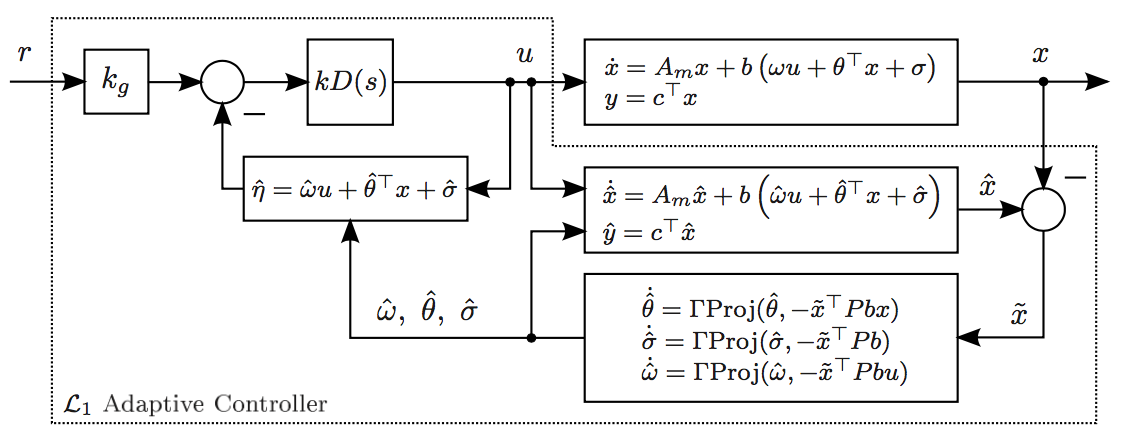
\includegraphics[width=0.75\textwidth]{L1_architecture.png}
  \caption{Generic $\mathcal{L}$1 Architecture}
  \label{fig:l1_architecture}
\end{figure}

The above simplified pitch model was used to illustrate how the following derivation is applied to the standard $x$ and $\dot{x}$ nomenclature as seen below.
\begin{equation}
\dot{x} =ax+bu
\end{equation}
ensuring that the DC gain is at unity, the equation becomes:
\begin{equation}
\dot{x} =-ax+au
\end{equation}
the error can be defined as
\begin{equation}
\tilde{x}=x-x_m
\end{equation}
therefore the derivative of the error becomes
\begin{equation}
\dot{\tilde{x}}=\dot{x}-\dot{x_m}
\end{equation}









